\documentclass[12pt]{article}

\usepackage[margin=1in]{geometry}
\usepackage{amsmath,amsthm,amssymb}
\usepackage{mathrsfs}
\usepackage{mathtools}
\usepackage{enumitem}
\usepackage{physics}
 
\usepackage{pdfpages}

\newcommand{\magsq}[1]{\big|#1\big|^2}
\newcommand{\avg}[1]{\left<#1\right>}

\begin{document}
	
\title{Homework 2}
\author{Sean Ericson \\ Phys 684}
\maketitle

\section*{Problem 1 {\small (Berman 2.9)}}
In the adiabatic approximation, the dressed-state amplitudes satisfy (eq. 2.146 in the textbook)
\begin{align*}
    c_{d_1}(t) &= e^{\frac{i}{2}\xi(t)}c_{d_1}(t_0) \\
    c_{d_2}(t) &= e^{-\frac{i}{2}\xi(t)}c_{d_2}(t_0),
\end{align*}
where 
\[ \xi(t) = \int_{t_0}^t \dd t' \Omega(t'). \]
In this case, $t_0 = -\infty$ and 
\[ \Omega_0(t) = \Omega_0e^{-\left(\frac{t}{T}\right)^2}, \]
so we can integrate that to get
\[ \xi(t) = \frac{\sqrt{\pi}}{2}\Omega_0T\left(1 + \erf\left(\frac{t}{T}\right)\right). \]
We transform between the dressed-states and the field-interaction basis states via
\[ \mqty(\tilde{c}_1\\\tilde{c}_2) = \mqty(c_\theta&s_\theta\\-s_\theta&c_\theta)\mqty(c_{d_1}\\c_{d_2}); \quad \mqty(c_{d_1}\\c_{d_2}) = \mqty(c_\theta&-s_\theta\\s_\theta&c_\theta)\mqty(\tilde{c}_1\\\tilde{c}_2), \]
where
\[ c_\theta = \sqrt{\frac{1}{2}\left(1 + \frac{\delta}{\Omega(t)}\right)}; \quad s_\theta = \sqrt{\frac{1}{2}\left(1 - \frac{\delta}{\Omega(t)}\right)}, \]
and $\Omega(t) = \sqrt{\delta^2 + \Omega_0^2(t)}$. Given that $\tilde{c}_1(-\infty) = 1$ and $\tilde{c}_2(-\infty)=0$, we find that
\begin{align*}
    c_{d_1}(-\infty) &= c_\theta(-\infty) = 1 \\
    c_{d_2}(-\infty) &= s_\theta(-\infty) = 0
\end{align*}
Putting everything together, we find
\begin{align*}
    \mqty(\tilde{c}_1(t)\\\tilde{c}_2(t)) &= \mqty(c_\theta&s_\theta\\-s_\theta&c_\theta)\mqty(c_{d_1}(t)\\c_{d_2}(t)) \\
    &= \mqty(c_\theta(t)c_{d_1}(t) + s_\theta(t)c_{d_2}(t) \\ -s_\theta c_{d_1}(t) + c_\theta c_{d_2}(t)) \\
    &= \mqty(c_\theta(t)\exp[\frac{i}{2}\xi(t)] \\ -s_\theta(t)\exp[\frac{i}{2}\xi(t)] )
\end{align*}


\section*{Problem 2 {\small (Berman 2.17)}}

\section*{Problem 3}
\begin{enumerate}[label=(\alph*)]
    \item Given that
    \[ H_0 = \hbar\mqty(\omega_1&0\\0&\omega_2), \]
    we have that
    \begin{align*}
        \exp(iH_0t/\hbar) &= \mqty(1&0\\0&1) + it\mqty(\omega_1&0\\0&\omega_2) + \frac{(it)^2}{2}\mqty(\omega_1&0\\0&\omega_2)^2 + \frac{(it)^3}{3!}\mqty(\omega_1&0\\0&\omega_2)^3 + \cdots \\
        &= \mqty(1 + i\omega_1t + \frac{1}{2}(i\omega_1t)^2 + \frac{1}{3!}(i\omega_1 t)^3 + \cdots & 0 \\ 0 & 1 + i\omega_2t + \frac{1}{2}(i\omega_2t)^2 + \frac{1}{3!}(i\omega_2t)^3 + \cdots) \\
        &= \mqty(\exp(i\omega_1t)&0\\0&\exp(i\omega_2t)).
    \end{align*}

    \item In the interaction representation, we factor out this free phase evolution by writing
    \[ \ket{\psi(t)}_\text{I} = \bar{c}_1(t)e^{-i\omega_1t}\ket{1} + \bar{c}_2(t)e^{-i\omega_2t}\ket{2}, \]
    that is, we make the (time-dependent) unitary transformation
    \[ \ket{\psi(t)}_\text{S} \to \ket{\psi(t)}_\text{I} = U(t)\ket{\psi(t)}_\text{S}, \]
    where
    \[ U(t) = \mqty(e^{-i\omega_1t}&0\\0&e^{-i\omega_2t}). \] 
    We get the effective interaction hamiltonian by making the inverse transformation on $V$:
    \[ V_\text{I} = U^\dag VU = \hbar\Omega_0 \cos(\omega t) \mqty(0&e^{-i\omega_0t}\\e^{i\omega_0t}&0), \]
    where the phase $\phi$ has been absorbed into the (complex) Rabi frequency.
\end{enumerate}

\section*{Problem 4}
We seek to find the eigenvectors of 
\[ \tilde{H} = \frac{\hbar}{2}\mqty(-\delta&\Omega_0\\\Omega_0&\delta). \]
Firstly, the eigenvalues of a 2x2 matrix are given by
\[ \frac{1}{2}\left(T \pm \sqrt{T^2 - 4D}\right), \]
where $T$ is the trace, and $D$ is the determinant. In this case,
\[ T = 0; \quad D = -\delta^2 - \Omega_0^2 \eqqcolon -\frac{\hbar^2\Omega^2}{4}, \]
so the eigenvalues are simply $\pm\frac{1}{2}\hbar\Omega$. Let the $+$ eigenvector be of the form
\[ \mqty(\sin\theta\\\cos\theta), \]
i.e.
\[ \frac{\hbar}{2}\mqty(-\delta&\Omega_0\\\Omega_0&\delta)\mqty(\sin\theta\\\cos\theta) = \frac{\hbar\Omega}{2}\mqty(\sin\theta\\\cos\theta). \]
Taking the first entry, we find
\begin{alignat*}{3}
    &\quad & -\delta\sin\theta + \Omega_0\cos\theta = \Omega\sin\theta \\
    &\implies\quad & (\Omega + \delta)\sin\theta &= \Omega_0\cos\theta \\
    &\implies\quad & \tan\theta = \frac{\Omega_0}{\Omega + \delta} \\
    &\implies\quad & \theta = \atan\frac{\Omega_0}{\Omega + \delta}.
\end{alignat*}
Now, using the identity
\[ \tan(2\atan(x)) = \frac{-2x}{x^2 - 1},  \]
we find
\begin{align*}
    \tan(2\theta) &= \frac{-2\left(\frac{\Omega_0}{\Omega + \delta}\right)}{\left(\frac{\Omega_0}{\Omega + \delta}\right)^2 - 1} \\
    &= \frac{\Omega_0}{\delta}.
\end{align*}
The eigenvectors are then
\begin{align*}
    \ket{+} &= \mqty(\sin\theta\\\cos\theta) \\
    \ket{-} &= \mqty(\cos\theta\\-\sin\theta),
\end{align*}
with $\theta$ given implicitly above.

\section*{Problem 4}
The general solution is given by
\[ \mqty(c_1(t)\\c_2(t)) = \mqty(e^{-i\delta t/2}\left[\left[\cos\frac{\Omega t}{2} + i\frac{\delta}{\Omega}\sin\frac{\Omega t}{2}\right]c_1(0) - i\frac{\Omega_0^*}{\Omega}\sin\frac{\Omega t}{2}c_2(0)\right] \\ e^{i\delta t/2}\left[-i\frac{\Omega_0}{\Omega}\sin\frac{\Omega t}{2}c_1(0) + \left[\cos\frac{\Omega t}{2} - i\frac{\delta}{\Omega}\sin\frac{\Omega t}{2}\right]c_2(0)\right]). \]
In the $\abs{\delta} \gg \Omega_0$ limit, we have that
\[ \Omega = \sqrt{\Omega_0^2 + \delta^2} \approx \delta(1 + \frac{\Omega_0^2}{\delta^2}) \]
\begin{enumerate}[label=(\alph*)]
    \item With the initial conditions $c_1(0) = 1$ and $c_2(0) = 0$, we have 
    \[ \mqty(c_1(t)\\c_2(t)) = \mqty(e^{-i\delta t/2}\left(\cos\frac{\Omega t}{2} + i\frac{\delta}{\Omega}\sin\frac{\Omega t}{2}\right)\\ -i\frac{\Omega_0}{\Omega}e^{i\delta t/2}\sin\frac{\Omega t}{2}) \]
\end{enumerate}
Focusing on $c_1$, we find
\begin{align*}
    c_1(t) &= e^{-i\delta t/2}\left(\cos\frac{\Omega t}{2} + i\frac{\delta}{\Omega}\sin\frac{\Omega t}{2}\right) \\
    &= \frac{1}{2}e^{-i\delta t/2}\left[\left(e^{i\Omega t/2} + e^{-i\Omega t/2}\right) + \frac{\delta}{\Omega}\left(e^{i\Omega t/2} - e^{-i\Omega t/2}\right)\right] \\
    &= \frac{1}{2\Omega}e^{-i(\delta+\Omega)t/2}\left[(\Omega - \delta) + (\Omega + \delta)e^{i\Omega t}\right] \\
    &= \frac{\Omega + \delta}{2\Omega}e^{-i(\delta-\Omega)t/2} + O(\frac{\Omega_0^2}{\delta^2}).
\end{align*}
Now, since this is in the interaction representation, we have that
\begin{align*}
    \ket{\psi(t)} &= c_1(t)e^{-i\omega_1t}\ket{1} \\
    &\propto e^{-i(\omega_1 + (\delta-\Omega)/2)t}\ket{1},
\end{align*}
i.e., the $\ket{1}$ state has an apparent energy shift of
\begin{align*}
    \Delta &= \frac{1}{2}(\delta - \Omega) \\
    &\approx \frac{1}{2}\left(\delta - \delta(1 - \frac{\Omega_0^2}{2\delta^2})\right) \\
    &= \frac{\Omega_0^2}{4\delta}
\end{align*}


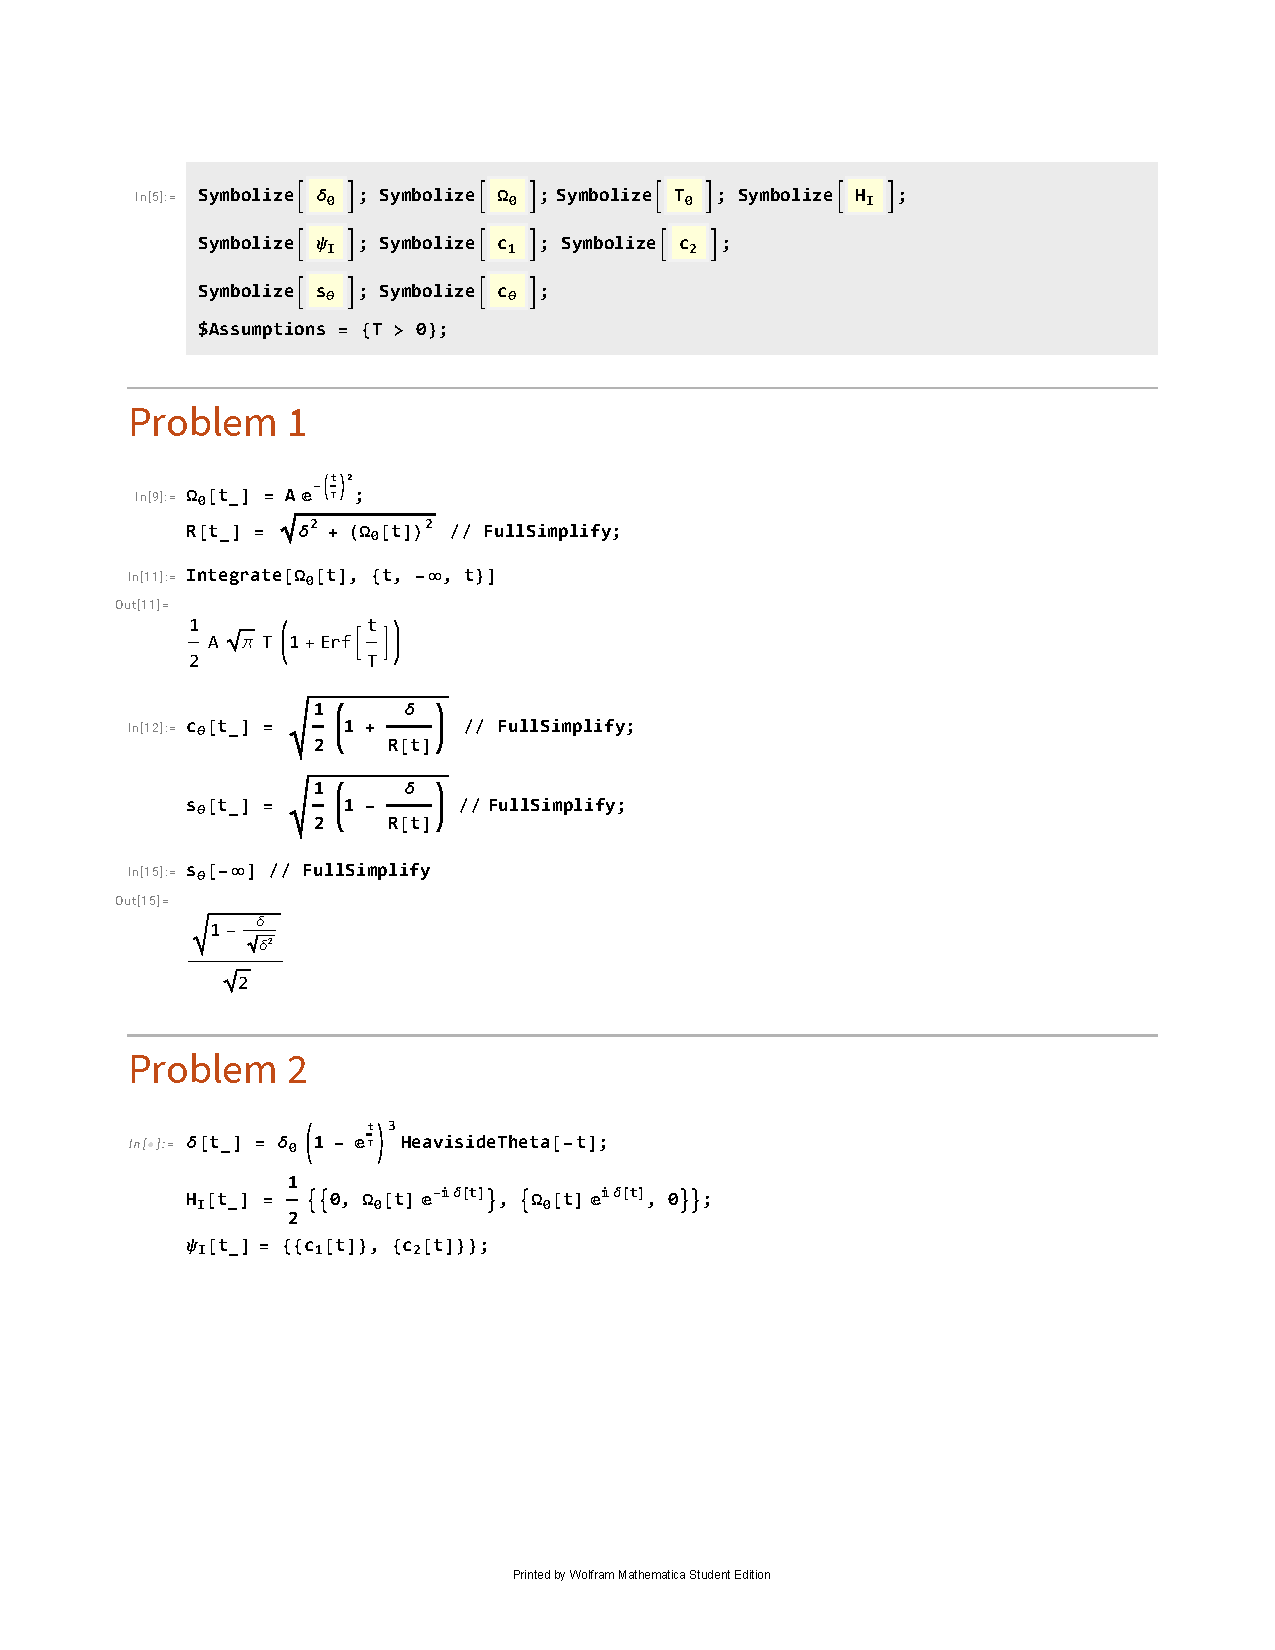
\includepdf[pages=-]{calcs/HW2_mathematica.pdf}
\end{document}